% generated by Plantuml 1.2025.7       
\definecolor{plantucolor0000}{RGB}{0,0,0}
\definecolor{plantucolor0001}{RGB}{255,255,255}
\definecolor{plantucolor0002}{RGB}{24,24,24}
\definecolor{plantucolor0003}{RGB}{226,226,240}
\definecolor{plantucolor0004}{RGB}{238,238,238}
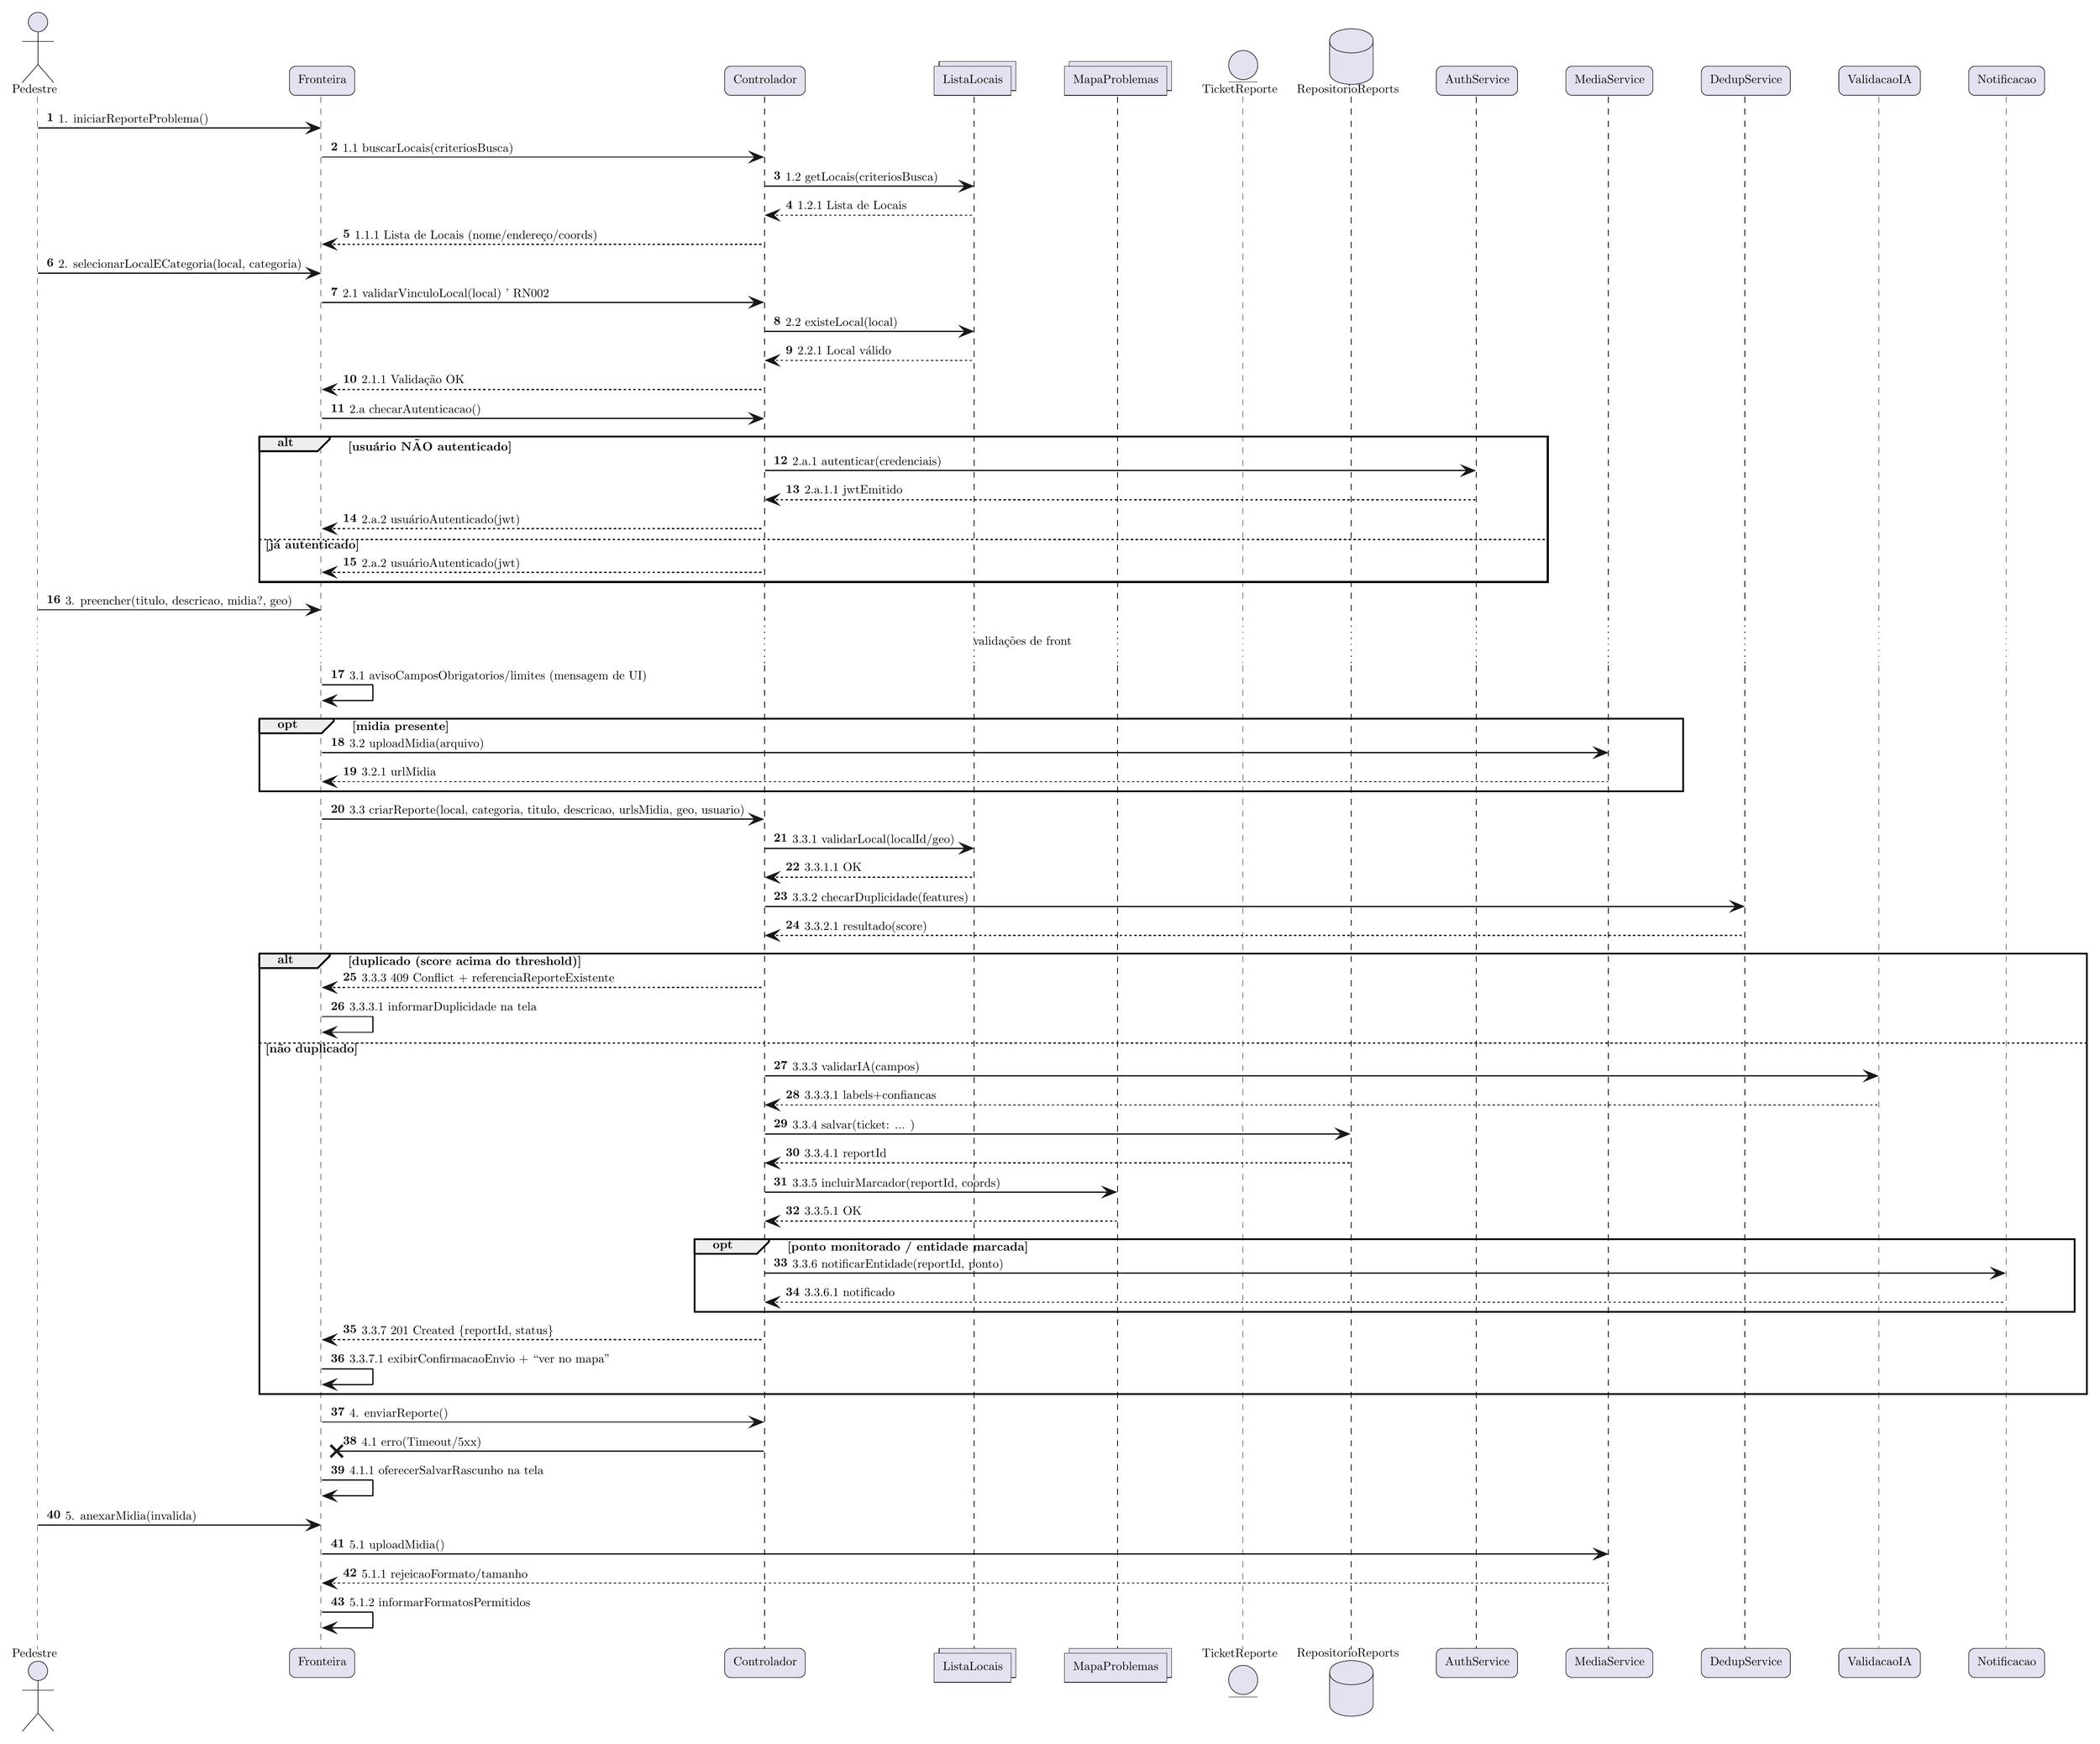
\begin{tikzpicture}[yscale=-1
,pstyle0/.style={color=black,line width=1.5pt}
,pstyle1/.style={color=plantucolor0001,line width=0.0pt}
,pstyle2/.style={color=plantucolor0002,line width=0.5pt,dash pattern=on 5.0pt off 5.0pt}
,pstyle3/.style={color=plantucolor0002,line width=0.5pt,dash pattern=on 1.0pt off 4.0pt}
,pstyle4/.style={color=plantucolor0002,fill=plantucolor0003,line width=0.5pt}
,pstyle5/.style={color=plantucolor0002,line width=0.5pt}
,pstyle6/.style={color=plantucolor0002,fill=plantucolor0002,line width=1.0pt}
,pstyle7/.style={color=plantucolor0002,line width=1.0pt}
,pstyle8/.style={color=plantucolor0002,line width=1.0pt,dash pattern=on 2.0pt off 2.0pt}
,pstyle9/.style={color=black,fill=plantucolor0004,line width=1.5pt}
,pstyle10/.style={color=black,line width=1.0pt,dash pattern=on 2.0pt off 2.0pt}
,pstyle11/.style={color=plantucolor0002,line width=2.0pt}
]
\draw[pstyle0] (209.335pt,356pt) rectangle (1273.8251pt,476pt);
\draw[pstyle0] (209.335pt,589pt) rectangle (1385.6351pt,649pt);
\draw[pstyle0] (209.335pt,783pt) rectangle (1719.2051pt,1147pt);
\draw[pstyle0] (568.8751pt,1019pt) rectangle (1709.2051pt,1079pt);
\draw[pstyle1] (22.58pt,75pt) rectangle (30.58pt,507pt);
\draw[pstyle2] (26pt,75pt) -- (26pt,507pt);
\draw[pstyle3] (26pt,507pt) -- (26pt,545pt);
\draw[pstyle1] (22.58pt,545pt) rectangle (30.58pt,1358pt);
\draw[pstyle2] (26pt,545pt) -- (26pt,1358pt);
\draw[pstyle1] (257.3pt,75pt) rectangle (265.3pt,507pt);
\draw[pstyle2] (260.335pt,75pt) -- (260.335pt,507pt);
\draw[pstyle3] (260.335pt,507pt) -- (260.335pt,545pt);
\draw[pstyle1] (257.3pt,545pt) rectangle (265.3pt,1358pt);
\draw[pstyle2] (260.335pt,545pt) -- (260.335pt,1358pt);
\draw[pstyle1] (623.1601pt,75pt) rectangle (631.1601pt,507pt);
\draw[pstyle2] (626.8751pt,75pt) -- (626.8751pt,507pt);
\draw[pstyle3] (626.8751pt,507pt) -- (626.8751pt,545pt);
\draw[pstyle1] (623.1601pt,545pt) rectangle (631.1601pt,1358pt);
\draw[pstyle2] (626.8751pt,545pt) -- (626.8751pt,1358pt);
\draw[pstyle1] (796.7301pt,75pt) rectangle (804.7301pt,507pt);
\draw[pstyle2] (799.9551pt,75pt) -- (799.9551pt,507pt);
\draw[pstyle3] (799.9551pt,507pt) -- (799.9551pt,545pt);
\draw[pstyle1] (796.7301pt,545pt) rectangle (804.7301pt,1358pt);
\draw[pstyle2] (799.9551pt,545pt) -- (799.9551pt,1358pt);
\draw[pstyle1] (914.7601pt,75pt) rectangle (922.7601pt,507pt);
\draw[pstyle2] (918.5051pt,75pt) -- (918.5051pt,507pt);
\draw[pstyle3] (918.5051pt,507pt) -- (918.5051pt,545pt);
\draw[pstyle1] (914.7601pt,545pt) rectangle (922.7601pt,1358pt);
\draw[pstyle2] (918.5051pt,545pt) -- (918.5051pt,1358pt);
\draw[pstyle1] (1018.2051pt,75pt) rectangle (1026.2051pt,507pt);
\draw[pstyle2] (1022.0151pt,75pt) -- (1022.0151pt,507pt);
\draw[pstyle3] (1022.0151pt,507pt) -- (1022.0151pt,545pt);
\draw[pstyle1] (1018.2051pt,545pt) rectangle (1026.2051pt,1358pt);
\draw[pstyle2] (1022.0151pt,545pt) -- (1022.0151pt,1358pt);
\draw[pstyle1] (1107.5651pt,75pt) rectangle (1115.5651pt,507pt);
\draw[pstyle2] (1111.3951pt,75pt) -- (1111.3951pt,507pt);
\draw[pstyle3] (1111.3951pt,507pt) -- (1111.3951pt,545pt);
\draw[pstyle1] (1107.5651pt,545pt) rectangle (1115.5651pt,1358pt);
\draw[pstyle2] (1111.3951pt,545pt) -- (1111.3951pt,1358pt);
\draw[pstyle1] (1211.2801pt,75pt) rectangle (1219.2801pt,507pt);
\draw[pstyle2] (1214.7351pt,75pt) -- (1214.7351pt,507pt);
\draw[pstyle3] (1214.7351pt,507pt) -- (1214.7351pt,545pt);
\draw[pstyle1] (1211.2801pt,545pt) rectangle (1219.2801pt,1358pt);
\draw[pstyle2] (1214.7351pt,545pt) -- (1214.7351pt,1358pt);
\draw[pstyle1] (1320.7301pt,75pt) rectangle (1328.7301pt,507pt);
\draw[pstyle2] (1323.8251pt,75pt) -- (1323.8251pt,507pt);
\draw[pstyle3] (1323.8251pt,507pt) -- (1323.8251pt,545pt);
\draw[pstyle1] (1320.7301pt,545pt) rectangle (1328.7301pt,1358pt);
\draw[pstyle2] (1323.8251pt,545pt) -- (1323.8251pt,1358pt);
\draw[pstyle1] (1433.4451pt,75pt) rectangle (1441.4451pt,507pt);
\draw[pstyle2] (1436.6351pt,75pt) -- (1436.6351pt,507pt);
\draw[pstyle3] (1436.6351pt,507pt) -- (1436.6351pt,545pt);
\draw[pstyle1] (1433.4451pt,545pt) rectangle (1441.4451pt,1358pt);
\draw[pstyle2] (1436.6351pt,545pt) -- (1436.6351pt,1358pt);
\draw[pstyle1] (1543.9251pt,75pt) rectangle (1551.9251pt,507pt);
\draw[pstyle2] (1547.2551pt,75pt) -- (1547.2551pt,507pt);
\draw[pstyle3] (1547.2551pt,507pt) -- (1547.2551pt,545pt);
\draw[pstyle1] (1543.9251pt,545pt) rectangle (1551.9251pt,1358pt);
\draw[pstyle2] (1547.2551pt,545pt) -- (1547.2551pt,1358pt);
\draw[pstyle1] (1648.9001pt,75pt) rectangle (1656.9001pt,507pt);
\draw[pstyle2] (1652.5951pt,75pt) -- (1652.5951pt,507pt);
\draw[pstyle3] (1652.5951pt,507pt) -- (1652.5951pt,545pt);
\draw[pstyle1] (1648.9001pt,545pt) rectangle (1656.9001pt,1358pt);
\draw[pstyle2] (1652.5951pt,545pt) -- (1652.5951pt,1358pt);
\node at (5pt,65pt)[below right,color=black,inner sep=0]{Pedestre};
\draw[pstyle4] (26.58pt,13.5pt) ellipse (8pt and 8pt);
\draw[pstyle5] (26.58pt,21.5pt) -- (26.58pt,48.5pt)(13.58pt,29.5pt) -- (39.58pt,29.5pt)(26.58pt,48.5pt) -- (13.58pt,63.5pt)(26.58pt,48.5pt) -- (39.58pt,63.5pt);
\node at (5pt,1357pt)[below right,color=black,inner sep=0]{Pedestre};
\draw[pstyle4] (26.58pt,1375.5pt) ellipse (8pt and 8pt);
\draw[pstyle5] (26.58pt,1383.5pt) -- (26.58pt,1410.5pt)(13.58pt,1391.5pt) -- (39.58pt,1391.5pt)(26.58pt,1410.5pt) -- (13.58pt,1425.5pt)(26.58pt,1410.5pt) -- (39.58pt,1425.5pt);
\draw[pstyle4] (234.335pt,55pt) arc (180:270:5pt) -- (239.335pt,50pt) -- (283.265pt,50pt) arc (270:360:5pt) -- (288.265pt,55pt) -- (288.265pt,69pt) arc (0:90:5pt) -- (283.265pt,74pt) -- (239.335pt,74pt) arc (90:180:5pt) -- (234.335pt,69pt) -- cycle;
\node at (241.335pt,57pt)[below right,color=black,inner sep=0]{Fronteira};
\draw[pstyle4] (234.335pt,1362pt) arc (180:270:5pt) -- (239.335pt,1357pt) -- (283.265pt,1357pt) arc (270:360:5pt) -- (288.265pt,1362pt) -- (288.265pt,1376pt) arc (0:90:5pt) -- (283.265pt,1381pt) -- (239.335pt,1381pt) arc (90:180:5pt) -- (234.335pt,1376pt) -- cycle;
\node at (241.335pt,1364pt)[below right,color=black,inner sep=0]{Fronteira};
\draw[pstyle4] (593.8751pt,55pt) arc (180:270:5pt) -- (598.8751pt,50pt) -- (655.4451pt,50pt) arc (270:360:5pt) -- (660.4451pt,55pt) -- (660.4451pt,69pt) arc (0:90:5pt) -- (655.4451pt,74pt) -- (598.8751pt,74pt) arc (90:180:5pt) -- (593.8751pt,69pt) -- cycle;
\node at (600.8751pt,57pt)[below right,color=black,inner sep=0]{Controlador};
\draw[pstyle4] (593.8751pt,1362pt) arc (180:270:5pt) -- (598.8751pt,1357pt) -- (655.4451pt,1357pt) arc (270:360:5pt) -- (660.4451pt,1362pt) -- (660.4451pt,1376pt) arc (0:90:5pt) -- (655.4451pt,1381pt) -- (598.8751pt,1381pt) arc (90:180:5pt) -- (593.8751pt,1376pt) -- cycle;
\node at (600.8751pt,1364pt)[below right,color=black,inner sep=0]{Controlador};
\draw[pstyle4] (770.9551pt,46pt) rectangle (834.5051pt,70pt);
\draw[pstyle4] (766.9551pt,50pt) rectangle (830.5051pt,74pt);
\node at (773.9551pt,57pt)[below right,color=black,inner sep=0]{ListaLocais};
\draw[pstyle4] (770.9551pt,1357pt) rectangle (834.5051pt,1381pt);
\draw[pstyle4] (766.9551pt,1361pt) rectangle (830.5051pt,1385pt);
\node at (773.9551pt,1368pt)[below right,color=black,inner sep=0]{ListaLocais};
\draw[pstyle4] (878.5051pt,46pt) rectangle (963.0151pt,70pt);
\draw[pstyle4] (874.5051pt,50pt) rectangle (959.0151pt,74pt);
\node at (881.5051pt,57pt)[below right,color=black,inner sep=0]{MapaProblemas};
\draw[pstyle4] (878.5051pt,1357pt) rectangle (963.0151pt,1381pt);
\draw[pstyle4] (874.5051pt,1361pt) rectangle (959.0151pt,1385pt);
\node at (881.5051pt,1368pt)[below right,color=black,inner sep=0]{MapaProblemas};
\node at (988.0151pt,65pt)[below right,color=black,inner sep=0]{TicketReporte};
\draw[pstyle4] (1022.2051pt,49pt) ellipse (12pt and 12pt);
\draw[pstyle5] (1010.2051pt,63pt) -- (1034.2051pt,63pt);
\node at (988.0151pt,1357pt)[below right,color=black,inner sep=0]{TicketReporte};
\draw[pstyle4] (1022.2051pt,1383pt) ellipse (12pt and 12pt);
\draw[pstyle5] (1010.2051pt,1397pt) -- (1034.2051pt,1397pt);
\node at (1066.3951pt,65pt)[below right,color=black,inner sep=0]{RepositorioReports};
\draw[pstyle4] (1093.5651pt,29pt) ..controls (1093.5651pt,19pt) and (1111.5651pt,19pt) .. (1111.5651pt,19pt) ..controls (1111.5651pt,19pt) and (1129.5651pt,19pt) .. (1129.5651pt,29pt) -- (1129.5651pt,55pt) ..controls (1129.5651pt,65pt) and (1111.5651pt,65pt) .. (1111.5651pt,65pt) ..controls (1111.5651pt,65pt) and (1093.5651pt,65pt) .. (1093.5651pt,55pt) -- (1093.5651pt,29pt);
\draw[pstyle5] (1093.5651pt,29pt) ..controls (1093.5651pt,39pt) and (1111.5651pt,39pt) .. (1111.5651pt,39pt) ..controls (1111.5651pt,39pt) and (1129.5651pt,39pt) .. (1129.5651pt,29pt);
\node at (1066.3951pt,1357pt)[below right,color=black,inner sep=0]{RepositorioReports};
\draw[pstyle4] (1093.5651pt,1377pt) ..controls (1093.5651pt,1367pt) and (1111.5651pt,1367pt) .. (1111.5651pt,1367pt) ..controls (1111.5651pt,1367pt) and (1129.5651pt,1367pt) .. (1129.5651pt,1377pt) -- (1129.5651pt,1403pt) ..controls (1129.5651pt,1413pt) and (1111.5651pt,1413pt) .. (1111.5651pt,1413pt) ..controls (1111.5651pt,1413pt) and (1093.5651pt,1413pt) .. (1093.5651pt,1403pt) -- (1093.5651pt,1377pt);
\draw[pstyle5] (1093.5651pt,1377pt) ..controls (1093.5651pt,1387pt) and (1111.5651pt,1387pt) .. (1111.5651pt,1387pt) ..controls (1111.5651pt,1387pt) and (1129.5651pt,1387pt) .. (1129.5651pt,1377pt);
\draw[pstyle4] (1181.7351pt,55pt) arc (180:270:5pt) -- (1186.7351pt,50pt) -- (1243.8251pt,50pt) arc (270:360:5pt) -- (1248.8251pt,55pt) -- (1248.8251pt,69pt) arc (0:90:5pt) -- (1243.8251pt,74pt) -- (1186.7351pt,74pt) arc (90:180:5pt) -- (1181.7351pt,69pt) -- cycle;
\node at (1188.7351pt,57pt)[below right,color=black,inner sep=0]{AuthService};
\draw[pstyle4] (1181.7351pt,1362pt) arc (180:270:5pt) -- (1186.7351pt,1357pt) -- (1243.8251pt,1357pt) arc (270:360:5pt) -- (1248.8251pt,1362pt) -- (1248.8251pt,1376pt) arc (0:90:5pt) -- (1243.8251pt,1381pt) -- (1186.7351pt,1381pt) arc (90:180:5pt) -- (1181.7351pt,1376pt) -- cycle;
\node at (1188.7351pt,1364pt)[below right,color=black,inner sep=0]{AuthService};
\draw[pstyle4] (1288.8251pt,55pt) arc (180:270:5pt) -- (1293.8251pt,50pt) -- (1355.6351pt,50pt) arc (270:360:5pt) -- (1360.6351pt,55pt) -- (1360.6351pt,69pt) arc (0:90:5pt) -- (1355.6351pt,74pt) -- (1293.8251pt,74pt) arc (90:180:5pt) -- (1288.8251pt,69pt) -- cycle;
\node at (1295.8251pt,57pt)[below right,color=black,inner sep=0]{MediaService};
\draw[pstyle4] (1288.8251pt,1362pt) arc (180:270:5pt) -- (1293.8251pt,1357pt) -- (1355.6351pt,1357pt) arc (270:360:5pt) -- (1360.6351pt,1362pt) -- (1360.6351pt,1376pt) arc (0:90:5pt) -- (1355.6351pt,1381pt) -- (1293.8251pt,1381pt) arc (90:180:5pt) -- (1288.8251pt,1376pt) -- cycle;
\node at (1295.8251pt,1364pt)[below right,color=black,inner sep=0]{MediaService};
\draw[pstyle4] (1400.6351pt,55pt) arc (180:270:5pt) -- (1405.6351pt,50pt) -- (1469.2551pt,50pt) arc (270:360:5pt) -- (1474.2551pt,55pt) -- (1474.2551pt,69pt) arc (0:90:5pt) -- (1469.2551pt,74pt) -- (1405.6351pt,74pt) arc (90:180:5pt) -- (1400.6351pt,69pt) -- cycle;
\node at (1407.6351pt,57pt)[below right,color=black,inner sep=0]{DedupService};
\draw[pstyle4] (1400.6351pt,1362pt) arc (180:270:5pt) -- (1405.6351pt,1357pt) -- (1469.2551pt,1357pt) arc (270:360:5pt) -- (1474.2551pt,1362pt) -- (1474.2551pt,1376pt) arc (0:90:5pt) -- (1469.2551pt,1381pt) -- (1405.6351pt,1381pt) arc (90:180:5pt) -- (1400.6351pt,1376pt) -- cycle;
\node at (1407.6351pt,1364pt)[below right,color=black,inner sep=0]{DedupService};
\draw[pstyle4] (1514.2551pt,55pt) arc (180:270:5pt) -- (1519.2551pt,50pt) -- (1576.5951pt,50pt) arc (270:360:5pt) -- (1581.5951pt,55pt) -- (1581.5951pt,69pt) arc (0:90:5pt) -- (1576.5951pt,74pt) -- (1519.2551pt,74pt) arc (90:180:5pt) -- (1514.2551pt,69pt) -- cycle;
\node at (1521.2551pt,57pt)[below right,color=black,inner sep=0]{ValidacaoIA};
\draw[pstyle4] (1514.2551pt,1362pt) arc (180:270:5pt) -- (1519.2551pt,1357pt) -- (1576.5951pt,1357pt) arc (270:360:5pt) -- (1581.5951pt,1362pt) -- (1581.5951pt,1376pt) arc (0:90:5pt) -- (1576.5951pt,1381pt) -- (1519.2551pt,1381pt) arc (90:180:5pt) -- (1514.2551pt,1376pt) -- cycle;
\node at (1521.2551pt,1364pt)[below right,color=black,inner sep=0]{ValidacaoIA};
\draw[pstyle4] (1621.5951pt,55pt) arc (180:270:5pt) -- (1626.5951pt,50pt) -- (1679.2051pt,50pt) arc (270:360:5pt) -- (1684.2051pt,55pt) -- (1684.2051pt,69pt) arc (0:90:5pt) -- (1679.2051pt,74pt) -- (1626.5951pt,74pt) arc (90:180:5pt) -- (1621.5951pt,69pt) -- cycle;
\node at (1628.5951pt,57pt)[below right,color=black,inner sep=0]{Notificacao};
\draw[pstyle4] (1621.5951pt,1362pt) arc (180:270:5pt) -- (1626.5951pt,1357pt) -- (1679.2051pt,1357pt) arc (270:360:5pt) -- (1684.2051pt,1362pt) -- (1684.2051pt,1376pt) arc (0:90:5pt) -- (1679.2051pt,1381pt) -- (1626.5951pt,1381pt) arc (90:180:5pt) -- (1621.5951pt,1376pt) -- cycle;
\node at (1628.5951pt,1364pt)[below right,color=black,inner sep=0]{Notificacao};
\draw[pstyle6] (249.3pt,97pt) -- (259.3pt,101pt) -- (249.3pt,105pt) -- (253.3pt,101pt) -- cycle;
\draw[pstyle7] (26.58pt,101pt) -- (255.3pt,101pt);
\node at (33.58pt,89pt)[below right,color=black,inner sep=0]{\textbf{1}};
\node at (43.33pt,89pt)[below right,color=black,inner sep=0]{1. iniciarReporteProblema()};
\draw[pstyle6] (615.1601pt,121pt) -- (625.1601pt,125pt) -- (615.1601pt,129pt) -- (619.1601pt,125pt) -- cycle;
\draw[pstyle7] (261.3pt,125pt) -- (621.1601pt,125pt);
\node at (268.3pt,113pt)[below right,color=black,inner sep=0]{\textbf{2}};
\node at (278.05pt,113pt)[below right,color=black,inner sep=0]{1.1 buscarLocais(criteriosBusca)};
\draw[pstyle6] (788.7301pt,145pt) -- (798.7301pt,149pt) -- (788.7301pt,153pt) -- (792.7301pt,149pt) -- cycle;
\draw[pstyle7] (627.1601pt,149pt) -- (794.7301pt,149pt);
\node at (634.1601pt,137pt)[below right,color=black,inner sep=0]{\textbf{3}};
\node at (643.9101pt,137pt)[below right,color=black,inner sep=0]{1.2 getLocais(criteriosBusca)};
\draw[pstyle6] (638.1601pt,169pt) -- (628.1601pt,173pt) -- (638.1601pt,177pt) -- (634.1601pt,173pt) -- cycle;
\draw[pstyle8] (632.1601pt,173pt) -- (799.7301pt,173pt);
\node at (644.1601pt,161pt)[below right,color=black,inner sep=0]{\textbf{4}};
\node at (653.9101pt,161pt)[below right,color=black,inner sep=0]{1.2.1 Lista de Locais};
\draw[pstyle6] (272.3pt,193pt) -- (262.3pt,197pt) -- (272.3pt,201pt) -- (268.3pt,197pt) -- cycle;
\draw[pstyle8] (266.3pt,197pt) -- (626.1601pt,197pt);
\node at (278.3pt,185pt)[below right,color=black,inner sep=0]{\textbf{5}};
\node at (288.05pt,185pt)[below right,color=black,inner sep=0]{1.1.1 Lista de Locais (nome/endereço/coords)};
\draw[pstyle6] (249.3pt,217pt) -- (259.3pt,221pt) -- (249.3pt,225pt) -- (253.3pt,221pt) -- cycle;
\draw[pstyle7] (26.58pt,221pt) -- (255.3pt,221pt);
\node at (33.58pt,209pt)[below right,color=black,inner sep=0]{\textbf{6}};
\node at (43.33pt,209pt)[below right,color=black,inner sep=0]{2. selecionarLocalECategoria(local, categoria)};
\draw[pstyle6] (615.1601pt,241pt) -- (625.1601pt,245pt) -- (615.1601pt,249pt) -- (619.1601pt,245pt) -- cycle;
\draw[pstyle7] (261.3pt,245pt) -- (621.1601pt,245pt);
\node at (268.3pt,233pt)[below right,color=black,inner sep=0]{\textbf{7}};
\node at (278.05pt,233pt)[below right,color=black,inner sep=0]{2.1 validarVinculoLocal(local)  ' RN002};
\draw[pstyle6] (788.7301pt,265pt) -- (798.7301pt,269pt) -- (788.7301pt,273pt) -- (792.7301pt,269pt) -- cycle;
\draw[pstyle7] (627.1601pt,269pt) -- (794.7301pt,269pt);
\node at (634.1601pt,257pt)[below right,color=black,inner sep=0]{\textbf{8}};
\node at (643.9101pt,257pt)[below right,color=black,inner sep=0]{2.2 existeLocal(local)};
\draw[pstyle6] (638.1601pt,289pt) -- (628.1601pt,293pt) -- (638.1601pt,297pt) -- (634.1601pt,293pt) -- cycle;
\draw[pstyle8] (632.1601pt,293pt) -- (799.7301pt,293pt);
\node at (644.1601pt,281pt)[below right,color=black,inner sep=0]{\textbf{9}};
\node at (653.9101pt,281pt)[below right,color=black,inner sep=0]{2.2.1 Local válido};
\draw[pstyle6] (272.3pt,313pt) -- (262.3pt,317pt) -- (272.3pt,321pt) -- (268.3pt,317pt) -- cycle;
\draw[pstyle8] (266.3pt,317pt) -- (626.1601pt,317pt);
\node at (278.3pt,305pt)[below right,color=black,inner sep=0]{\textbf{10}};
\node at (293.8pt,305pt)[below right,color=black,inner sep=0]{2.1.1 Validação OK};
\draw[pstyle6] (615.1601pt,337pt) -- (625.1601pt,341pt) -- (615.1601pt,345pt) -- (619.1601pt,341pt) -- cycle;
\draw[pstyle7] (261.3pt,341pt) -- (621.1601pt,341pt);
\node at (268.3pt,329pt)[below right,color=black,inner sep=0]{\textbf{11}};
\node at (283.8pt,329pt)[below right,color=black,inner sep=0]{2.a checarAutenticacao()};
\draw[pstyle9] (209.335pt,356pt) -- (267.585pt,356pt) -- (267.585pt,358pt) -- (257.585pt,368pt) -- (209.335pt,368pt) -- (209.335pt,356pt);
\draw[pstyle0] (209.335pt,356pt) rectangle (1273.8251pt,476pt);
\node at (224.335pt,357pt)[below right,color=black,inner sep=0]{\textbf{alt}};
\node at (282.585pt,358pt)[below right,color=black,inner sep=0]{\textbf{[usuário NÃO autenticado]}};
\draw[pstyle6] (1203.2801pt,380pt) -- (1213.2801pt,384pt) -- (1203.2801pt,388pt) -- (1207.2801pt,384pt) -- cycle;
\draw[pstyle7] (627.1601pt,384pt) -- (1209.2801pt,384pt);
\node at (634.1601pt,372pt)[below right,color=black,inner sep=0]{\textbf{12}};
\node at (649.6601pt,372pt)[below right,color=black,inner sep=0]{2.a.1 autenticar(credenciais)};
\draw[pstyle6] (638.1601pt,404pt) -- (628.1601pt,408pt) -- (638.1601pt,412pt) -- (634.1601pt,408pt) -- cycle;
\draw[pstyle8] (632.1601pt,408pt) -- (1214.2801pt,408pt);
\node at (644.1601pt,396pt)[below right,color=black,inner sep=0]{\textbf{13}};
\node at (659.6601pt,396pt)[below right,color=black,inner sep=0]{2.a.1.1 jwtEmitido};
\draw[pstyle6] (272.3pt,428pt) -- (262.3pt,432pt) -- (272.3pt,436pt) -- (268.3pt,432pt) -- cycle;
\draw[pstyle8] (266.3pt,432pt) -- (626.1601pt,432pt);
\node at (278.3pt,420pt)[below right,color=black,inner sep=0]{\textbf{14}};
\node at (293.8pt,420pt)[below right,color=black,inner sep=0]{2.a.2 usuárioAutenticado(jwt)};
\draw[pstyle10] (209.335pt,441pt) -- (1273.8251pt,441pt);
\node at (214.335pt,441pt)[below right,color=black,inner sep=0]{\textbf{[já autenticado]}};
\draw[pstyle6] (272.3pt,464pt) -- (262.3pt,468pt) -- (272.3pt,472pt) -- (268.3pt,468pt) -- cycle;
\draw[pstyle8] (266.3pt,468pt) -- (626.1601pt,468pt);
\node at (278.3pt,456pt)[below right,color=black,inner sep=0]{\textbf{15}};
\node at (293.8pt,456pt)[below right,color=black,inner sep=0]{2.a.2 usuárioAutenticado(jwt)};
\draw[pstyle6] (249.3pt,495pt) -- (259.3pt,499pt) -- (249.3pt,503pt) -- (253.3pt,499pt) -- cycle;
\draw[pstyle7] (26.58pt,499pt) -- (255.3pt,499pt);
\node at (33.58pt,487pt)[below right,color=black,inner sep=0]{\textbf{16}};
\node at (49.08pt,487pt)[below right,color=black,inner sep=0]{3. preencher(titulo, descricao, midia?, geo)};
\node at (795.535pt,521pt)[below right,color=black,inner sep=0]{~validações de front~};
\draw[pstyle7] (261.3pt,561pt) -- (303.3pt,561pt);
\draw[pstyle7] (303.3pt,561pt) -- (303.3pt,574pt);
\draw[pstyle7] (262.3pt,574pt) -- (303.3pt,574pt);
\draw[pstyle6] (272.3pt,570pt) -- (262.3pt,574pt) -- (272.3pt,578pt) -- (268.3pt,574pt) -- cycle;
\node at (268.3pt,549pt)[below right,color=black,inner sep=0]{\textbf{17}};
\node at (283.8pt,549pt)[below right,color=black,inner sep=0]{3.1 avisoCamposObrigatorios/limites (mensagem de UI)};
\draw[pstyle9] (209.335pt,589pt) -- (270.945pt,589pt) -- (270.945pt,591pt) -- (260.945pt,601pt) -- (209.335pt,601pt) -- (209.335pt,589pt);
\draw[pstyle0] (209.335pt,589pt) rectangle (1385.6351pt,649pt);
\node at (224.335pt,590pt)[below right,color=black,inner sep=0]{\textbf{opt}};
\node at (285.945pt,591pt)[below right,color=black,inner sep=0]{\textbf{[midia presente]}};
\draw[pstyle6] (1312.7301pt,613pt) -- (1322.7301pt,617pt) -- (1312.7301pt,621pt) -- (1316.7301pt,617pt) -- cycle;
\draw[pstyle7] (261.3pt,617pt) -- (1318.7301pt,617pt);
\node at (268.3pt,605pt)[below right,color=black,inner sep=0]{\textbf{18}};
\node at (283.8pt,605pt)[below right,color=black,inner sep=0]{3.2 uploadMidia(arquivo)};
\draw[pstyle6] (272.3pt,637pt) -- (262.3pt,641pt) -- (272.3pt,645pt) -- (268.3pt,641pt) -- cycle;
\draw[pstyle8] (266.3pt,641pt) -- (1323.7301pt,641pt);
\node at (278.3pt,629pt)[below right,color=black,inner sep=0]{\textbf{19}};
\node at (293.8pt,629pt)[below right,color=black,inner sep=0]{3.2.1 urlMidia};
\draw[pstyle6] (615.1601pt,668pt) -- (625.1601pt,672pt) -- (615.1601pt,676pt) -- (619.1601pt,672pt) -- cycle;
\draw[pstyle7] (261.3pt,672pt) -- (621.1601pt,672pt);
\node at (268.3pt,660pt)[below right,color=black,inner sep=0]{\textbf{20}};
\node at (283.8pt,660pt)[below right,color=black,inner sep=0]{3.3 criarReporte(local, categoria, titulo, descricao, urlsMidia, geo, usuario)};
\draw[pstyle6] (788.7301pt,692pt) -- (798.7301pt,696pt) -- (788.7301pt,700pt) -- (792.7301pt,696pt) -- cycle;
\draw[pstyle7] (627.1601pt,696pt) -- (794.7301pt,696pt);
\node at (634.1601pt,684pt)[below right,color=black,inner sep=0]{\textbf{21}};
\node at (649.6601pt,684pt)[below right,color=black,inner sep=0]{3.3.1 validarLocal(localId/geo)};
\draw[pstyle6] (638.1601pt,716pt) -- (628.1601pt,720pt) -- (638.1601pt,724pt) -- (634.1601pt,720pt) -- cycle;
\draw[pstyle8] (632.1601pt,720pt) -- (799.7301pt,720pt);
\node at (644.1601pt,708pt)[below right,color=black,inner sep=0]{\textbf{22}};
\node at (659.6601pt,708pt)[below right,color=black,inner sep=0]{3.3.1.1 OK};
\draw[pstyle6] (1425.4451pt,740pt) -- (1435.4451pt,744pt) -- (1425.4451pt,748pt) -- (1429.4451pt,744pt) -- cycle;
\draw[pstyle7] (627.1601pt,744pt) -- (1431.4451pt,744pt);
\node at (634.1601pt,732pt)[below right,color=black,inner sep=0]{\textbf{23}};
\node at (649.6601pt,732pt)[below right,color=black,inner sep=0]{3.3.2 checarDuplicidade(features)};
\draw[pstyle6] (638.1601pt,764pt) -- (628.1601pt,768pt) -- (638.1601pt,772pt) -- (634.1601pt,768pt) -- cycle;
\draw[pstyle8] (632.1601pt,768pt) -- (1436.4451pt,768pt);
\node at (644.1601pt,756pt)[below right,color=black,inner sep=0]{\textbf{24}};
\node at (659.6601pt,756pt)[below right,color=black,inner sep=0]{3.3.2.1 resultado(score)};
\draw[pstyle9] (209.335pt,783pt) -- (267.585pt,783pt) -- (267.585pt,785pt) -- (257.585pt,795pt) -- (209.335pt,795pt) -- (209.335pt,783pt);
\draw[pstyle0] (209.335pt,783pt) rectangle (1719.2051pt,1147pt);
\node at (224.335pt,784pt)[below right,color=black,inner sep=0]{\textbf{alt}};
\node at (282.585pt,785pt)[below right,color=black,inner sep=0]{\textbf{[duplicado (score acima do threshold)]}};
\draw[pstyle6] (272.3pt,807pt) -- (262.3pt,811pt) -- (272.3pt,815pt) -- (268.3pt,811pt) -- cycle;
\draw[pstyle8] (266.3pt,811pt) -- (626.1601pt,811pt);
\node at (278.3pt,799pt)[below right,color=black,inner sep=0]{\textbf{25}};
\node at (293.8pt,799pt)[below right,color=black,inner sep=0]{3.3.3 409 Conflict + referenciaReporteExistente};
\draw[pstyle7] (261.3pt,835pt) -- (303.3pt,835pt);
\draw[pstyle7] (303.3pt,835pt) -- (303.3pt,848pt);
\draw[pstyle7] (262.3pt,848pt) -- (303.3pt,848pt);
\draw[pstyle6] (272.3pt,844pt) -- (262.3pt,848pt) -- (272.3pt,852pt) -- (268.3pt,848pt) -- cycle;
\node at (268.3pt,823pt)[below right,color=black,inner sep=0]{\textbf{26}};
\node at (283.8pt,823pt)[below right,color=black,inner sep=0]{3.3.3.1 informarDuplicidade na tela};
\draw[pstyle10] (209.335pt,857pt) -- (1719.2051pt,857pt);
\node at (214.335pt,857pt)[below right,color=black,inner sep=0]{\textbf{[não duplicado]}};
\draw[pstyle6] (1535.9251pt,880pt) -- (1545.9251pt,884pt) -- (1535.9251pt,888pt) -- (1539.9251pt,884pt) -- cycle;
\draw[pstyle7] (627.1601pt,884pt) -- (1541.9251pt,884pt);
\node at (634.1601pt,872pt)[below right,color=black,inner sep=0]{\textbf{27}};
\node at (649.6601pt,872pt)[below right,color=black,inner sep=0]{3.3.3 validarIA(campos)};
\draw[pstyle6] (638.1601pt,904pt) -- (628.1601pt,908pt) -- (638.1601pt,912pt) -- (634.1601pt,908pt) -- cycle;
\draw[pstyle8] (632.1601pt,908pt) -- (1546.9251pt,908pt);
\node at (644.1601pt,896pt)[below right,color=black,inner sep=0]{\textbf{28}};
\node at (659.6601pt,896pt)[below right,color=black,inner sep=0]{3.3.3.1 labels+confiancas};
\draw[pstyle6] (1099.5651pt,928pt) -- (1109.5651pt,932pt) -- (1099.5651pt,936pt) -- (1103.5651pt,932pt) -- cycle;
\draw[pstyle7] (627.1601pt,932pt) -- (1105.5651pt,932pt);
\node at (634.1601pt,920pt)[below right,color=black,inner sep=0]{\textbf{29}};
\node at (649.6601pt,920pt)[below right,color=black,inner sep=0]{3.3.4 salvar(ticket: ... )};
\draw[pstyle6] (638.1601pt,952pt) -- (628.1601pt,956pt) -- (638.1601pt,960pt) -- (634.1601pt,956pt) -- cycle;
\draw[pstyle8] (632.1601pt,956pt) -- (1110.5651pt,956pt);
\node at (644.1601pt,944pt)[below right,color=black,inner sep=0]{\textbf{30}};
\node at (659.6601pt,944pt)[below right,color=black,inner sep=0]{3.3.4.1 reportId};
\draw[pstyle6] (906.7601pt,976pt) -- (916.7601pt,980pt) -- (906.7601pt,984pt) -- (910.7601pt,980pt) -- cycle;
\draw[pstyle7] (627.1601pt,980pt) -- (912.7601pt,980pt);
\node at (634.1601pt,968pt)[below right,color=black,inner sep=0]{\textbf{31}};
\node at (649.6601pt,968pt)[below right,color=black,inner sep=0]{3.3.5 incluirMarcador(reportId, coords)};
\draw[pstyle6] (638.1601pt,1000pt) -- (628.1601pt,1004pt) -- (638.1601pt,1008pt) -- (634.1601pt,1004pt) -- cycle;
\draw[pstyle8] (632.1601pt,1004pt) -- (917.7601pt,1004pt);
\node at (644.1601pt,992pt)[below right,color=black,inner sep=0]{\textbf{32}};
\node at (659.6601pt,992pt)[below right,color=black,inner sep=0]{3.3.5.1 OK};
\draw[pstyle9] (568.8751pt,1019pt) -- (630.4851pt,1019pt) -- (630.4851pt,1021pt) -- (620.4851pt,1031pt) -- (568.8751pt,1031pt) -- (568.8751pt,1019pt);
\draw[pstyle0] (568.8751pt,1019pt) rectangle (1709.2051pt,1079pt);
\node at (583.8751pt,1020pt)[below right,color=black,inner sep=0]{\textbf{opt}};
\node at (645.4851pt,1021pt)[below right,color=black,inner sep=0]{\textbf{[ponto monitorado / entidade marcada]}};
\draw[pstyle6] (1640.9001pt,1043pt) -- (1650.9001pt,1047pt) -- (1640.9001pt,1051pt) -- (1644.9001pt,1047pt) -- cycle;
\draw[pstyle7] (627.1601pt,1047pt) -- (1646.9001pt,1047pt);
\node at (634.1601pt,1035pt)[below right,color=black,inner sep=0]{\textbf{33}};
\node at (649.6601pt,1035pt)[below right,color=black,inner sep=0]{3.3.6 notificarEntidade(reportId, ponto)};
\draw[pstyle6] (638.1601pt,1067pt) -- (628.1601pt,1071pt) -- (638.1601pt,1075pt) -- (634.1601pt,1071pt) -- cycle;
\draw[pstyle8] (632.1601pt,1071pt) -- (1651.9001pt,1071pt);
\node at (644.1601pt,1059pt)[below right,color=black,inner sep=0]{\textbf{34}};
\node at (659.6601pt,1059pt)[below right,color=black,inner sep=0]{3.3.6.1 notificado};
\draw[pstyle6] (272.3pt,1098pt) -- (262.3pt,1102pt) -- (272.3pt,1106pt) -- (268.3pt,1102pt) -- cycle;
\draw[pstyle8] (266.3pt,1102pt) -- (626.1601pt,1102pt);
\node at (278.3pt,1090pt)[below right,color=black,inner sep=0]{\textbf{35}};
\node at (293.8pt,1090pt)[below right,color=black,inner sep=0]{3.3.7 201 Created \{reportId, status\}};
\draw[pstyle7] (261.3pt,1126pt) -- (303.3pt,1126pt);
\draw[pstyle7] (303.3pt,1126pt) -- (303.3pt,1139pt);
\draw[pstyle7] (262.3pt,1139pt) -- (303.3pt,1139pt);
\draw[pstyle6] (272.3pt,1135pt) -- (262.3pt,1139pt) -- (272.3pt,1143pt) -- (268.3pt,1139pt) -- cycle;
\node at (268.3pt,1114pt)[below right,color=black,inner sep=0]{\textbf{36}};
\node at (283.8pt,1114pt)[below right,color=black,inner sep=0]{3.3.7.1 exibirConfirmacaoEnvio + ``ver no mapa''};
\draw[pstyle6] (615.1601pt,1166pt) -- (625.1601pt,1170pt) -- (615.1601pt,1174pt) -- (619.1601pt,1170pt) -- cycle;
\draw[pstyle7] (261.3pt,1170pt) -- (621.1601pt,1170pt);
\node at (268.3pt,1158pt)[below right,color=black,inner sep=0]{\textbf{37}};
\node at (283.8pt,1158pt)[below right,color=black,inner sep=0]{4. enviarReporte()};
\draw[pstyle11] (268.3pt,1189pt) -- (278.3pt,1199pt);
\draw[pstyle11] (268.3pt,1199pt) -- (278.3pt,1189pt);
\draw[pstyle7] (273.3pt,1194pt) -- (626.1601pt,1194pt);
\node at (278.3pt,1182pt)[below right,color=black,inner sep=0]{\textbf{38}};
\node at (293.8pt,1182pt)[below right,color=black,inner sep=0]{4.1 erro(Timeout/5xx)};
\draw[pstyle7] (261.3pt,1218pt) -- (303.3pt,1218pt);
\draw[pstyle7] (303.3pt,1218pt) -- (303.3pt,1231pt);
\draw[pstyle7] (262.3pt,1231pt) -- (303.3pt,1231pt);
\draw[pstyle6] (272.3pt,1227pt) -- (262.3pt,1231pt) -- (272.3pt,1235pt) -- (268.3pt,1231pt) -- cycle;
\node at (268.3pt,1206pt)[below right,color=black,inner sep=0]{\textbf{39}};
\node at (283.8pt,1206pt)[below right,color=black,inner sep=0]{4.1.1 oferecerSalvarRascunho na tela};
\draw[pstyle6] (249.3pt,1251pt) -- (259.3pt,1255pt) -- (249.3pt,1259pt) -- (253.3pt,1255pt) -- cycle;
\draw[pstyle7] (26.58pt,1255pt) -- (255.3pt,1255pt);
\node at (33.58pt,1243pt)[below right,color=black,inner sep=0]{\textbf{40}};
\node at (49.08pt,1243pt)[below right,color=black,inner sep=0]{5. anexarMidia(invalida)};
\draw[pstyle6] (1312.7301pt,1275pt) -- (1322.7301pt,1279pt) -- (1312.7301pt,1283pt) -- (1316.7301pt,1279pt) -- cycle;
\draw[pstyle7] (261.3pt,1279pt) -- (1318.7301pt,1279pt);
\node at (268.3pt,1267pt)[below right,color=black,inner sep=0]{\textbf{41}};
\node at (283.8pt,1267pt)[below right,color=black,inner sep=0]{5.1 uploadMidia()};
\draw[pstyle6] (272.3pt,1299pt) -- (262.3pt,1303pt) -- (272.3pt,1307pt) -- (268.3pt,1303pt) -- cycle;
\draw[pstyle8] (266.3pt,1303pt) -- (1323.7301pt,1303pt);
\node at (278.3pt,1291pt)[below right,color=black,inner sep=0]{\textbf{42}};
\node at (293.8pt,1291pt)[below right,color=black,inner sep=0]{5.1.1 rejeicaoFormato/tamanho};
\draw[pstyle7] (261.3pt,1327pt) -- (303.3pt,1327pt);
\draw[pstyle7] (303.3pt,1327pt) -- (303.3pt,1340pt);
\draw[pstyle7] (262.3pt,1340pt) -- (303.3pt,1340pt);
\draw[pstyle6] (272.3pt,1336pt) -- (262.3pt,1340pt) -- (272.3pt,1344pt) -- (268.3pt,1340pt) -- cycle;
\node at (268.3pt,1315pt)[below right,color=black,inner sep=0]{\textbf{43}};
\node at (283.8pt,1315pt)[below right,color=black,inner sep=0]{5.1.2 informarFormatosPermitidos};
\end{tikzpicture}
